\documentclass[spec, och, labwork]{shiza}
% параметр - тип обучения - одно из значений:
%    spec     - специальность
%    bachelor - бакалавриат (по умолчанию)
%    master   - магистратура
% параметр - форма обучения - одно из значений:
%    och   - очное (по умолчанию)
%    zaoch - заочное
% параметр - тип работы - одно из значений:
%    referat    - реферат
%    coursework - курсовая работа (по умолчанию)
%    diploma    - дипломная работа
%    pract      - отчет по практике
% параметр - включение шрифта
%    times    - включение шрифта Times New Roman (если установлен)
%               по умолчанию выключен
\usepackage{subfigure}
\usepackage{tikz,pgfplots}
\pgfplotsset{compat=1.5}
\usepackage{float}

%\usepackage{titlesec}
\setcounter{secnumdepth}{4}
%\titleformat{\paragraph}
%{\normalfont\normalsize}{\theparagraph}{1em}{}
%\titlespacing*{\paragraph}
%{35.5pt}{3.25ex plus 1ex minus .2ex}{1.5ex plus .2ex}

\titleformat{\paragraph}[block]
{\hspace{1.25cm}\normalfont}
{\theparagraph}{1ex}{}
\titlespacing{\paragraph}
{0cm}{2ex plus 1ex minus .2ex}{.4ex plus.2ex}

% --------------------------------------------------------------------------%


\usepackage[T2A]{fontenc}
\usepackage[utf8]{inputenc}
\usepackage{graphicx}
\graphicspath{ {./images/} }
\usepackage{tempora}

\usepackage[sort,compress]{cite}
\usepackage{amsmath}
\usepackage{amssymb}
\usepackage{amsthm}
\usepackage{fancyvrb}
\usepackage{listings}
\usepackage{listingsutf8}
\usepackage{longtable}
\usepackage{array}
\usepackage[english,russian]{babel}

% \usepackage[colorlinks=true]{hyperref}
\usepackage{url}

\usepackage{underscore}
\usepackage{setspace}
\usepackage{indentfirst} 
\usepackage{mathtools}
\usepackage{amsfonts}
\usepackage{enumitem}
\usepackage{tikz}
\usepackage{minted}

\newcommand{\eqdef}{\stackrel {\rm def}{=}}
\newcommand{\specialcell}[2][c]{%
\begin{tabular}[#1]{@{}c@{}}#2\end{tabular}}

\renewcommand\theFancyVerbLine{\small\arabic{FancyVerbLine}}

\newtheorem{lem}{Лемма}

\begin{document}

% Кафедра (в родительном падеже)
\chair{}

% Тема работы
\title{Классификация бинарных отношений и системы замыканий}

% Курс
\course{3}

% Группа
\group{331}

% Факультет (в родительном падеже) (по умолчанию "факультета КНиИТ")
\department{факультета КНиИТ}

% Специальность/направление код - наименование
%\napravlenie{09.03.04 "--- Программная инженерия}
%\napravlenie{010500 "--- Математическое обеспечение и администрирование информационных систем}
%\napravlenie{230100 "--- Информатика и вычислительная техника}
%\napravlenie{231000 "--- Программная инженерия}
\napravlenie{100501 "--- Компьютерная безопасность}

% Для студентки. Для работы студента следующая команда не нужна.
% \studenttitle{Студентки}

% Фамилия, имя, отчество в родительном падеже
\author{Окунькова Сергея Викторовича}

% Заведующий кафедрой
% \chtitle{} % степень, звание
% \chname{}

%Научный руководитель (для реферата преподаватель проверяющий работу)
\satitle{аспирант} %должность, степень, звание
\saname{В. Н. Кутин}

% Руководитель практики от организации (только для практики,
% для остальных типов работ не используется)
% \patitle{к.ф.-м.н.}
% \paname{С.~В.~Миронов}

% Семестр (только для практики, для остальных
% типов работ не используется)
%\term{8}

% Наименование практики (только для практики, для остальных
% типов работ не используется)
%\practtype{преддипломная}

% Продолжительность практики (количество недель) (только для практики,
% для остальных типов работ не используется)
%\duration{4}

% Даты начала и окончания практики (только для практики, для остальных
% типов работ не используется)
%\practStart{30.04.2019}
%\practFinish{27.05.2019}

% Год выполнения отчета
\date{2022}

\maketitle

% Включение нумерации рисунков, формул и таблиц по разделам
% (по умолчанию - нумерация сквозная)
% (допускается оба вида нумерации)
% \secNumbering

%-------------------------------------------------------------------------------------------
\tableofcontents

\section{Постановка задачи}

Цель работы:

Изучение основных свойств бинарных отношений и операций замыкания бинарных отношений.

Порядок выполнения работы:
    \begin{enumerate}
        \item Рассмотреть понятия полугруппы, подполугруппы и порождающего множества. Разработать алгоритм построения подполугрупп по по таблице Кэли.
        \item Разработать алгоритм построения полугруппы бинарных отношений по заданному порождающему множеству.
        \item Рассмотреть понятия подгруппы, порождающего множества и определяющих соотношений. Разработать алгоритм построения полугруппы по порождающему
        множеству и определяющим соотношениям.
    \end{enumerate}

\section{Теоретические сведения по рассмотренным темам с их обоснованием}

\textbf{Полугруппа} – это алгебра $S = (S, \cdot)$ с однойассоциативной бинарной операцией $\cdot$, т.е. выполняется
$(x \cdot y) \cdot z = x \cdot (y \cdot z)$ для любых $x,y,z \in S$.

Если полугрупповая операция называется умножением (соответственно, сложением), то полугруппу называют мультипликативной
(соответственно, аддитивной).

Подмножество X полугруппы S называется \textbf{подполугруппой}, если X устойчиво относительно операции умножения, т.е. для любых
$x, y \in X$ выполняется свойство: $x \cdot y \in X$.

В этом случае множество X с ограничением на нем операции умножения исходной полугруппы S образует полугруппу.

В силу общего свойства подалгебр пересечение любого семейства $X_i$ $(i \in I)$ подполугрупп полугруппы $S$ является
подполугруппой $S$ и, значит, множество $Sub(S)$ всех подполугрупп полугруппы $S$ является системой замыканий.
множество $X$. Такая полугруппа обозначается символом $\langle X \rangle$ и называется подполугруппой $S$, порождённой множеством
$X$. При этом множество $X$ называется также \textbf{порождающим множеством} подполугруппы $\langle X \rangle$. В частности, если
$\langle X \rangle = S$, то $X$ называется порождающим множеством полугруппы $S$ и говорят, что множество $X$ порождает полугруппу
$S$.

Для любой конечной полугруппы S найдется такой конечный алфавит A, что для некоторого отображения
$\phi : A \rightarrow S$ выполняется равенство $<\phi(A)>=S$ и, значит, $S \cong A^+/ ker \phi$ этом случае множество A
называется множеством порождающих символов полугруппы S (относительно отображения $\phi : A \rightarrow S$ ). Если
при этом для слов $w_1,w_2 \in A$ выполняется равенство $\phi(w_1) = \phi(w_2)$, т.е. $w_1 \equiv w_2(ker\phi)$ , то
говорят, что на S выполняется соотношение $w_1 = w_2$ (относительно отображения $\phi : A \rightarrow S$).

Очевидно, что в общем случае множество таких соотношений $w_1 = w_2$ для всех пар $(w_1, w_2) \in ker\phi$ будет бесконечным
и не представляется возможности эффективно описать полугруппу S в виде полугруппы классов конгруэнции $ker\phi$ . Однако в
некоторых случаях можно выбрать такое сравнительно простое подмножество $\rho \subset ker\phi$ , которое однозначно определяет
конгруэнцию $ker\phi$ как наименьшую конгруэнцию полугруппы $A^+$ , содержащую отношение $\rho$, т.е. $ker\phi = f_{con}(\rho) = f_{eq}(f_{reg}(\rho))$.

Так как в случае $(w_1, w_2) \in \rho$ по-прежнему выполняется равенство $\phi(w_1) = \phi(w_2)$, то будем писать
$w_1 = w_2$ и называть такие выражения \textbf{определяющими соотношениями}. Из таких соотношений конгруэнция $ker\phi$ строится
с помощью применения следующих процедур к словам $u,v \in A^+$ :

(а) слово $v$ непосредственно выводится из слова $u$, если $v$ получается из $u$ заменой некоторого подслова $w_1$ на слово
$w_2$, удовлетворяющее определяющему соотношению $w_1 = w_2$, т.е. $(u, v) = (xw_1y, xw_2y)$ для некоторых $x, y \in A^*$;

(б) слово $v$ выводится из слова $u$, если $v$ получается из $u$ с помощью конечного числа применения процедуры (а).

Если все выполняющиеся на $S$ соотношения выводятся из определяющих соотношений совокупности $\rho$, то конгруэнция $ker\phi$
полностью определяется отношением $\rho$ и выражение $<A: {w_1 = w_2 : (w_1, w_2) \in \rho}>$ называется \textbf{копредставлением полугруппы $S$}.

\section{Результаты работы}

    \subsection{Алгоритм 1 - Построение подполугруппы по заданному порождающему множеству}

        \textit{Вход}: Полугруппа $S$ с таблицей Кэли $A = (a_{ij})$ размерности $n \times n$ и подмножество $X \subset S$.

        \textit{Выход}: Подполугруппа $\langle X \rangle \subset S$.\\
        \underline{Шаг 1.} Положим $i = 0$, $X_0 = X$.\\
        \underline{Шаг 2.} Для $X_i$ вычислим $\overline{X}_l = \{x \cdot y : x \in X_i \wedge y \in X \}$ и положим $X_{i + 1} = X_i \cup \overline{X}_l$ (выражение $x \cdot y$ означает $a_{xy}$ в таблице Кэли $A$). \\
        \underline{Шаг 3.} Если $X_{i + 1} = X_i$ вернем $X_i$, которое будет являться подполугруппой $\langle X \rangle \subset S$, иначе положим $i=i+1$ и вернемся ко 2-му шагу.
    
        Трудоемкость алгоритма $O(n^3)$.

    \subsection{Алгоритм 2 - Построение полугруппы бинарных отношений по заданному порождающему множеству}

        \textit{Вход}: Конечное множество $X$ бинарных отношений, заданное булевыми матрицами размерности $n \times n$.

        \textit{Выход}: Полугруппа $\langle X \rangle$.\\
        \underline{Шаг 1.} Необходимо инициализировать список $matrices = []$. Известно, что каждому элементу $x_i \in X$ ($0 \leq i < n$)
        соответствует матрица $A_i \in M$, где $M$ -- множество матриц $A_i$ ($0 \leq i < n$), тогда элементы списка $matrices$ будут
        заданы следующим образом: $matrices[i] = A_i$ ($0 \leq i < n$). Стоит отметить, что список $matrices$ есть полугруппа $\langle X \rangle$.\\
        \underline{Шаг 2.} Необходимо создать список $combinations$, элементы которого будут $c_k \in combinations$, где $0 \leq k < (n^1 + n^2 + ... + n^n)$.
        Т.е. этот список является суммой размещений с повторениями.\\
        \underline{Шаг 3.} Далее возьмем матрицу $A_i$ ($0 \leq i < n$) и умножим ее на матрицы $B_0, ..., B_l$ согласно текущей комбинации $c_k$ 
        ($0 \leq k < (n^1 + n^2 + ... + n^n)$), где матрицы $B_1, ..., B_l \in M$ составляют текущую комбинацию $c_k$ ($l$ -- количество элементов в $c_k$).
        Таким образом получаем матрицу $C = A_i \odot B_1 \odot \dots \odot B_l$, где $\odot$ -- операция поэлементного умножения. 
        Добавляем $C$ в список $matrices$ в качестве нового элемента полугруппы $\langle X \rangle$.\\
        \underline{Шаг 4.} Повторять шаг 3 $k$ раз ($0 \leq k < (n^1 + n^2 + ... + n^n)$). \\

        Трудоемкость алгоритма $O(m^n)$.\\
    \subsection{Алгоритм 3 - Построение полугруппы по порождающему множеству и определяющим соотношениям}

        \textit{Вход}: Конечное множество символов $A$ размерности $n$ и конечное множество $R$ определяющих соотношений размерности $m \times n$.

        \textit{Выход}: Полугруппа $\langle A | R \rangle$.\\
        \underline{Шаг 1.} Необходимо инициализировать пустой список $gl$ и добавить в него все элементы генератора $R$.
        Инициализировать массив $alph = gl$\\
        \underline{Шаг 2.} К каждому элемента $gl$ добавить каждый элемент $alph$ и посчитать новое определяющее соотношение.
        Оно будет рассчитываться как массив, размерности $n$, где k элемент $(0 \leq k < n)$ будет равен $R[i][j]$, где i -
        это добавленный элемент из $alph$, а j - позиция k-го элемента в $A$.\\
        \underline{Шаг 3.} Если все полученные значения соотношений уже есть в $R$, вернуть $R$, иначе $gl = $ все уникальные соотношения
        и вернуться к шагу 2.

        Трудоемкость алгоритма $O(m^n)$.\\
    
        \subsection{Коды программ, реализующей рассмотренные алгоритмы}
            \inputminted[fontsize=\small]{python}{../code/lab4.py}
        \subsection{Результаты тестирования программ}

        \begin{figure}[H]
            \centering      %размер рисунка       здесь находится название файла рисунка, без указания формата
            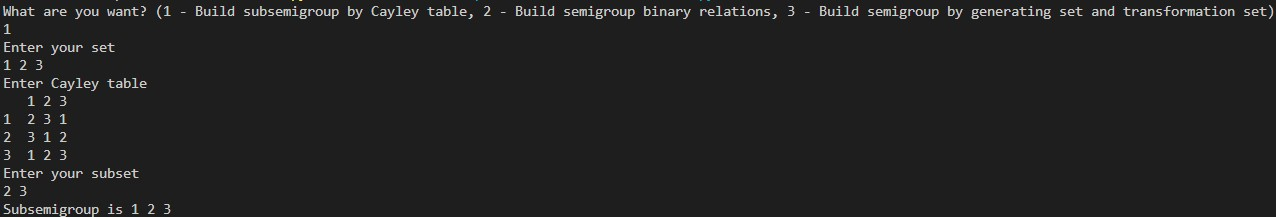
\includegraphics[width=1.\textwidth]{pic/1}
            \caption{Тест алгоритма построения подполугрупп по по таблице Кэли}
            \label{fig:image1}
        \end{figure}

        \begin{figure}[H]
            \centering      %размер рисунка       здесь находится название файла рисунка, без указания формата
            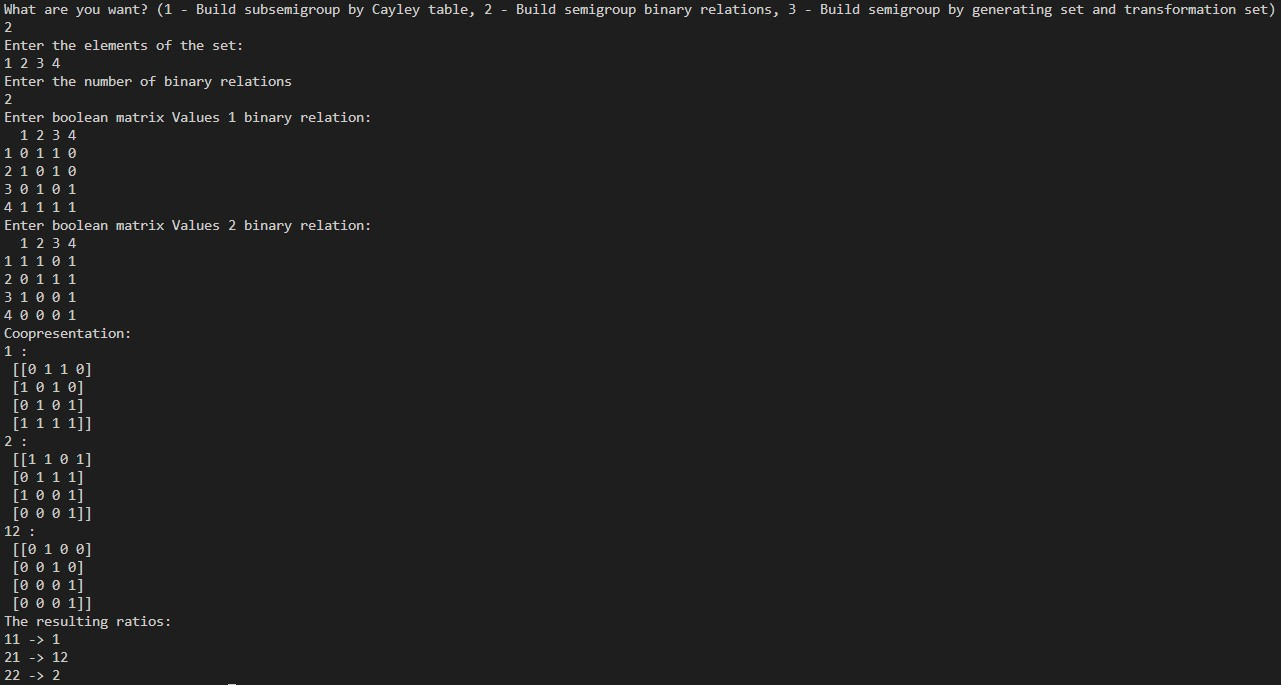
\includegraphics[width=1.\textwidth]{pic/2}
            \caption{Тест алгоритма построения полугруппы бинарных отношений по
            заданному порождающему множеству}
            \label{fig:image1}
        \end{figure}

        \begin{figure}[H]
            \centering      %размер рисунка       здесь находится название файла рисунка, без указания формата
            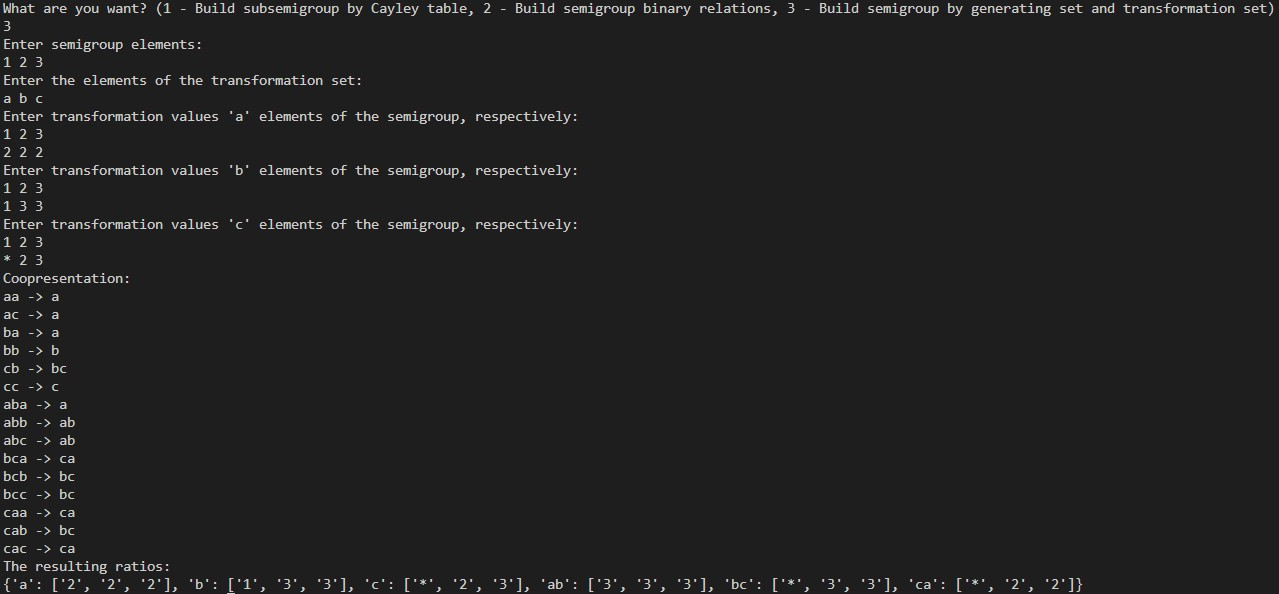
\includegraphics[width=1.\textwidth]{pic/3}
            \caption{Тест алгоритма построения полугруппы по порождающему
            множеству и определяющим соотношениям}
            \label{fig:image1}
        \end{figure}

        \subsection{Ответы на задачи}

        % \begin{figure}[H]
        %     \centering
        %     \includegraphics[width=0.8\textwidth]{pic/task1.png}
        %     \caption{Ответ на задачу 1}
        % \end{figure}

        \textbf{Задание 1.} Найдите полугруппу S = $\langle f, g \rangle$ преобразований множества $X = {1, 2, 3}$,
        порожденную следующими преобразованиями $f, g$ в симметрической полугруппе $T(X)$ преобразований множества $X$:
        \begin{center}
          $f = \begin{pmatrix}
            1 & 2 & 3 \\
            3 & 3 & 3
        \end{pmatrix}$,
          $g = \begin{pmatrix}
            1 & 2 & 3 \\
            3 & 1 & 2
          \end{pmatrix}$.
        \end{center}

      Известно, что множество преобразований $f, g$ порождает полугруппу S = $\langle f, g \rangle$ преобразований
      множества X, которая состоит из элементов $f, g, f^2 , f g, gf, g^2 , \dots $ и является подполугруппой конечной
      полугруппы $T(X)$.
  
      $f^2 = 
      \begin{pmatrix}
        1 & 2 & 3 \\
        3 & 3 & 3
      \end{pmatrix} \cdot
      \begin{pmatrix}
        1 & 2 & 3 \\
        3 & 3 & 3
      \end{pmatrix} = 
      \begin{tabular}{c c c c}
        & 1 & 2 & 3 \\
        f & $\downarrow$ & $\downarrow$ & $\downarrow$ \\
        & 3 & 3 & 3 \\
        f & $\downarrow$ & $\downarrow$ & $\downarrow$ \\
        & 3 & 3 & 3 \\
      \end{tabular} = 
      \begin{pmatrix}
        1 & 2 & 3 \\
        3 & 3 & 3
      \end{pmatrix}$
  
      $fg = 
      \begin{pmatrix}
        1 & 2 & 3 \\
        3 & 3 & 3
      \end{pmatrix} \cdot
      \begin{pmatrix}
        1 & 2 & 3 \\
        3 & 1 & 2
      \end{pmatrix} = 
      \begin{tabular}{c c c c}
        & 1 & 2 & 3 \\
        f & $\downarrow$ & $\downarrow$ & $\downarrow$ \\
        & 3 & 3 & 3 \\
        g & $\downarrow$ & $\downarrow$ & $\downarrow$ \\
        & 2 & 2 & 2 \\
      \end{tabular} = 
      \begin{pmatrix}
        1 & 2 & 3 \\
        2 & 2 & 2
      \end{pmatrix}$
  
      $g^2 = 
      \begin{pmatrix}
        1 & 2 & 3 \\
        3 & 1 & 2
      \end{pmatrix} \cdot
      \begin{pmatrix}
        1 & 2 & 3 \\
        3 & 1 & 2
      \end{pmatrix} = 
      \begin{tabular}{c c c c}
        & 1 & 2 & 3 \\
        g & $\downarrow$ & $\downarrow$ & $\downarrow$ \\
        & 3 & 1 & 2 \\
        g & $\downarrow$ & $\downarrow$ & $\downarrow$ \\
        & 2 & 3 & 1 \\
      \end{tabular} = 
      \begin{pmatrix}
        1 & 2 & 3 \\
        2 & 3 & 1
      \end{pmatrix}$
  
      $g^3 = 
      \begin{pmatrix}
        1 & 2 & 3 \\
        2 & 3 & 1
      \end{pmatrix} \cdot
      \begin{pmatrix}
        1 & 2 & 3 \\
        3 & 1 & 2
      \end{pmatrix} = 
      \begin{tabular}{c c c c}
        & 1 & 2 & 3 \\
        gg & $\downarrow$ & $\downarrow$ & $\downarrow$ \\
        & 2 & 3 & 1 \\
        g & $\downarrow$ & $\downarrow$ & $\downarrow$ \\
        & 1 & 2 & 3 \\
      \end{tabular} = 
      \begin{pmatrix}
        1 & 2 & 3 \\
        1 & 2 & 3
      \end{pmatrix}$

      $fg^2 = 
      \begin{pmatrix}
        1 & 2 & 3 \\
        2 & 2 & 2
      \end{pmatrix} \cdot
      \begin{pmatrix}
        1 & 2 & 3 \\
        3 & 1 & 2
      \end{pmatrix} = 
      \begin{tabular}{c c c c}
        & 1 & 2 & 3 \\
        fg & $\downarrow$ & $\downarrow$ & $\downarrow$ \\
        & 2 & 2 & 2 \\
        g & $\downarrow$ & $\downarrow$ & $\downarrow$ \\
        & 1 & 1 & 1 \\
      \end{tabular} = 
      \begin{pmatrix}
        1 & 2 & 3 \\
        1 & 1 & 1
      \end{pmatrix}$

      \textbf{Задание 2.} Найдите индекс и период следующих элементов a полугруппы преобразований
      множества X={1,2,3,4,5}:

      \begin{center}
        $a = \begin{pmatrix}
          1 & 2 & 3 & 4 & 5\\
          3 & 1 & 1 & 2 & 2
      \end{pmatrix}$
      \end{center}

      \begin{center}
        $aa = \begin{pmatrix}
          1 & 2 & 3 & 4 & 5\\
          1 & 3 & 3 & 1 & 1
      \end{pmatrix}$
      \end{center}

      \begin{center}
        $aaa = \begin{pmatrix}
          1 & 2 & 3 & 4 & 5\\
          3 & 1 & 1 & 3 & 3
      \end{pmatrix}$
      \end{center}

      \begin{center}
        $aaaa = \begin{pmatrix}
          1 & 2 & 3 & 4 & 5\\
          1 & 3 & 3 & 1 & 1
      \end{pmatrix}$
      \end{center}

        Видно, что $aaaa \rightarrow aa$. Т. е. период будет равен 2.
        \textbf{Задание 3.} Найдите полугруппу S по ее копредставлению $\langle x, y : xy = yx, x^3 = x^2, y^2 = y
        \rangle$. Выделим полную систему представителей классов конгруэнции $\varepsilon$, которая определяется
        соотношениями данного копредставления. Для этого последовательно рассмотрим слова фиксированной длины и выделим
        те, которые не будут эквивалентны между собой относительно конгруэнции $\varepsilon$.

        Сначала рассматриваем слова длины $1$: $x, y$ - эти слова не эквивалентны между собой относительно конгруэнции
        $\varepsilon$.

        Затем рассматриваем слова длины $2$, которые получаются из слов длины $1$ путем последовательного умножения их
        справа на буквы $x$ и $y$: $x^2 = x$, $xy$, $yx = xy$, $y^2$ - из этих слов только слова $y^2$, $xy$ не
        эквивалентны относительно конгруэнции $\varepsilon$ другим ранее выделенным словам.

        Теперь рассматриваем слова длины $3$, которые получаются из выделенных слов длины $2$ путем последовательного
        умножения их справа на буквы $x$ и $y$: $y^3 = y$, $xy^2 = y^2x$, $xyx = x^2y = xy$, $xy^2$ – из этих слов только
        слово $xy^2$ не эквивалентно относительно конгруэнции $\varepsilon$ другим ранее выделенным словам.

        Наконец рассматриваем слова длины $4$, которые получаются из выделенного слова длины $3$ путем последовательного
        умножения его справа на буквы $x$ и $y$: $xy^2x = x^2y^2 = xy^2$, $xy^3 = xy$ - все эти слова эквивалентны
        относительно конгруэнции $\varepsilon$ ранее выделенным словам.

        Значит, $S = \{x, y, y^2, xy, xy^2 \}$ "--- полная система представителей классов конгруэнции $\varepsilon$.
        Операция умножения $\cdot$ таких слов определяется с точностью до конгруэнции $\varepsilon$ по следующей таблице
        Кэли:
        
        \begin{table}[h]
          \begin{center}
          \begin{tabular}{|l|l|l|l|l|l|}
          \hline
          $\cdot $ & $x$ & $y$  & $xy$  & $y^2$ & $xy^2$ \\ \hline
          $x$      & $x$ & $xy$ & $xy$  & $xy^2$ & $xy^2$ \\ \hline
          $y$      & $xy$& $y^2$ & $xy^2$ & $y$ & $xy$ \\ \hline
          $xy$    & $xy$ & $xy^2$ & $xy^2$ & $xy$ & $xy$ \\ \hline
          $y^2$     &$xy^2$& $y$ & $xy$ & $y^2$ & $xy^2$ \\ \hline
          $xy^2y$   & $xy^2$ &  $xy$  &  $xy$ & $xy^2$ & $xy^2$ \\ \hline
          \end{tabular}
          \end{center}
        \end{table}


\conclusion

В рамках данной лабораторной работы были рассмотренны теоритические основы свойств бинарных подгруп и полугрупп, а также способы
их построения. На основе этой теоретической части была смоделирована программа на языке Python с 
использованием средств библиотеки Numpy, которая способна построить подполугрупп по по таблице Кэли, построить полугруппу
бинарных отношений по заданному порождающему множеству и построить полугруппу по порождающему множеству и определяющим соотношениям.

\end{document}
